%versi 3 (22-07-2020)

\chapter{Landasan Teori}
\label{chap:teori}

\section{Aplikasi Rugby Indonesia}
\label{sec:skripsi} 
    Aplikasi Rugby Indonesia merupakan aplikasi resmi dari Persatuan Rugby Union Indonesia yang dapat memberikan informasi terbaru mengenai olahraga \textit{rugby} di Indonesia. Aplikasi ini dapat memberikan notifikasi langsung mengenai berita terakhir, turnamen yang akan datang, dan informasi lainnya. Selain itu, aplikasi ini juga memungkinkan pengguna untuk mengambil gambar dan menunjukkan dukungan mereka dengan rekan-rekan penggemar \textit{rugby} lainnya dengan meng-\textit{upload} gambar ke dalam halaman \textit{Teammate Photos}. Terdapat juga aplikasi multimedia pengenalan olahraga \textit{rugby} berbasis Android yang dapat memberikan informasi sejarah, peraturan, dan peralatan serta tempat-latihan \textit{rugby} di beberapa Kabupaten/Kota. Aplikasi Rugby Indonesia tersedia di Google Play Store dan dapat diunduh secara gratis. Gambar dari halaman Rugby Indonesia dapat dilihat pada Gambar \ref{fig:rugby-halaman-label}.

    % \begin{figure} [!h]
    %     \centering
    %     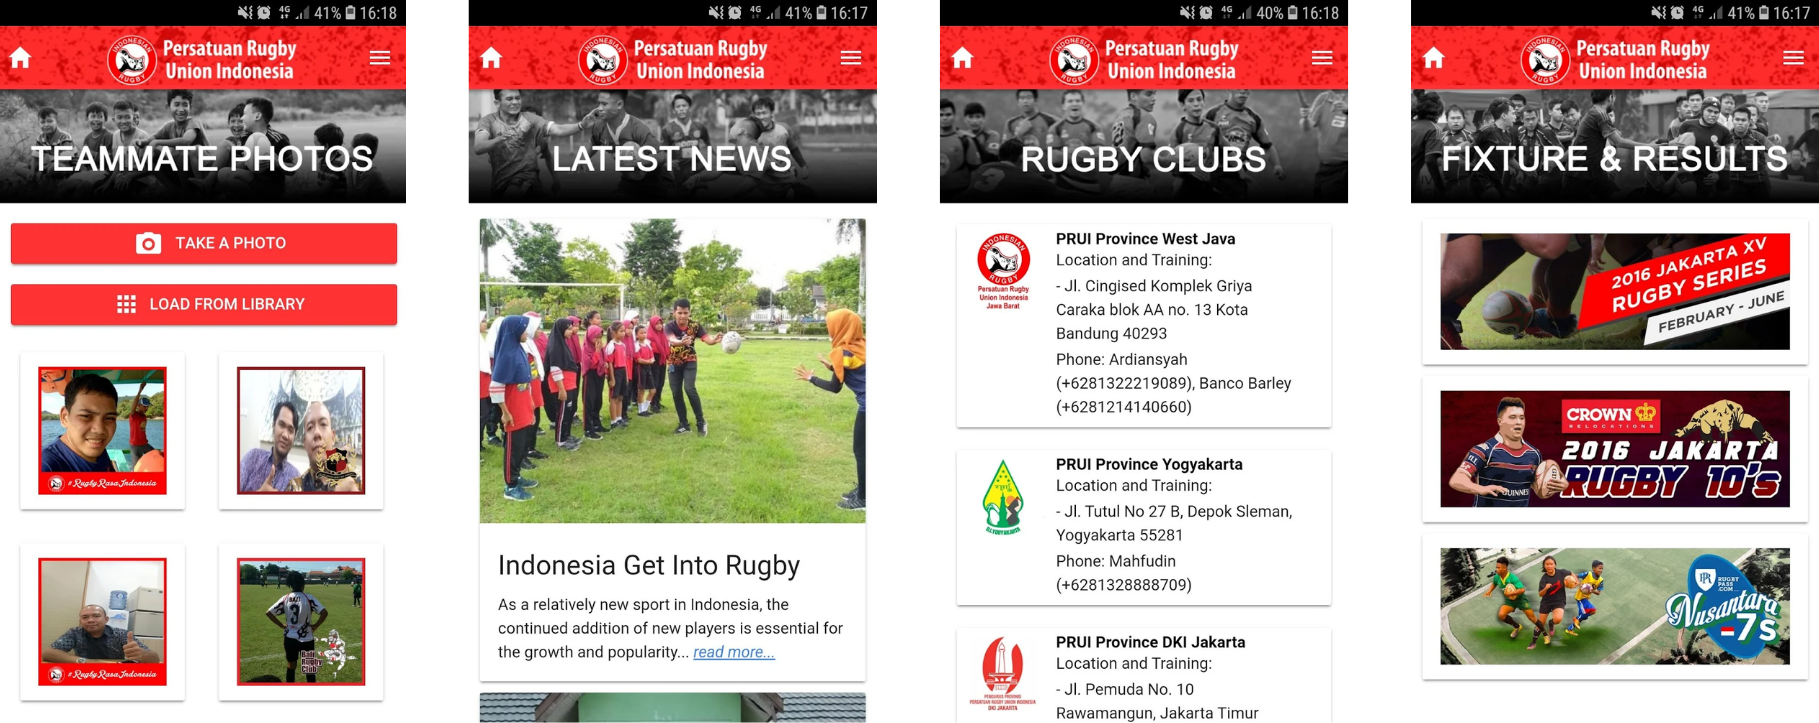
\includegraphics[scale=0.725]{Gambar/Rugby-Indonesia-App-UI.png}
    %     \caption[Halaman aplikasi Rugby Indonesia]{Halaman-halaman dari aplikasi Rugby Indonesia}
    %     \label{fig:halaman-rugby-indonesia}
    % \end{figure}

    Fitur-fitur yang ada pada aplikasi Rugby Indonesia dengan versi terakhir yang ada saat ini yaitu:

    \begin{enumerate}
        \item Halaman \textit{Latest News} yang diambil dari \url{https://rugbyindonesia.or.id/berita/} dengan memanfaatkan protokol RSS. 
        \item Halaman \textit{Fixture \& Results}.
        \item Halaman \textit{Teammate Photos} dengan fungsi:
        \begin{itemize}
            \item Pengguna dapat langsung mengambil foto dari aplikasi tersebut.
            \item Pengguna dapat langsung memberikan \textit{frame} terhadap foto tersebut.
            \item Pengguna dapat langsung menggunggah foto tersebut ke dalam galeri publik.
        \end{itemize}
    \item Halaman \textit{Rugby Clubs} yang memiliki fungsi di mana pengguna dapat langsung mendaftar ke dalam \textit{Rugby Clubs} yang berada di Indonesia.
    \item Fungsi \textit{Push Notifications}.
    \end{enumerate}
    
\section{\texorpdfstring{ReactJS~\cite{react-docs}}{ReactJS}}
\label{sec:reactJS}

ReactJS atau React adalah sebuah \textit{library} JavaScript yang digunakan untuk membangun \textit{user interface} yang interaktif. ReactJS berisi kumpulan potongan kode JavaScript yang disebut ``komponen'' yang bisa digunakan berulang kali untuk mendesain antarmuka pengguna. ReactJS bukanlah \textit{framework} JavaScript, karena hanya bertugas untuk me-\textit{render} komponen area tampilan aplikasi. ReactJS dapat digunakan untuk membuat aplikasi web dan \textit{mobile}.

\subsection{Hooks}
\label{subsec:hooks}
Hooks adalah fitur yang memungkinkan penggunaan \textit{state} dan fitur React lainnya tanpa membuat sebuah kelas. Hooks berfungsi untuk ``mengaitkan'' \textit{state} dan fitur-fitur \textit{lifecycle} React dari \textit{function component}.

\subsubsection{State Hooks}
\label{subsubsec:state-hooks}
State Hooks adalah salah satu jenis Hooks yang memungkinkan pengembang untuk menggunakan \textit{state} pada \textit{function component} tanpa harus membuat sebuah kelas. Cara untuk menggunakan State Hooks terdapat pada (Kode \ref{kode:state-hooks-example}), di mana `useState' digunakan untuk mendeklarasikan sebuah variabel \textit{state} yang dapat langsung di \textit{update}.
\begin{lstlisting}[language=HTML, caption=Contoh Potongan Kode State Hooks, label=kode:state-hooks-example]
function ImageGallery() {
  const [index, setIndex] = useState(0);
  // ...
\end{lstlisting}

\subsubsection{Context Hooks}
\label{subsubsec:context-hooks}
Context Hooks adalah salah satu jenis Hooks yang memungkinkan pengembang untuk menerima informasi dari \textit{parent} yang jauh tanpa meneruskannya sebagai properti. Cara untuk menggunakan Context Hooks terdapat pada (Kode \ref{kode:context-hooks-example}). Pada kode tersebut, `useContext' digunakan untuk berlangganan pada sebuah \textit{context} yang berada pada komponen.
\begin{lstlisting}[language=HTML, caption=Contoh Potongan Kode Context Hooks, label=kode:context-hooks-example]
function Button() {
  const theme = useContext(ThemeContext);
  // ...
\end{lstlisting}

\subsubsection{Ref Hooks}
\label{subsubsec:ref-hooks}
Ref Hook pada React adalah salah satu dari beberapa Hooks bawaan yang memungkinkan penggunaan \textit{refs} dalam komponen fungsional. \textit{Ref} digunakan untuk mengakses DOM atau nilai dari elemen \textit{child} dalam React. Cara untuk menggunakan Ref Hooks terdapat pada (Kode \ref{kode:ref-hooks-example}). Pada kode tersebut, `useRef' digunakan untuk mereferensikan sebuah nilai yang tidak digunakan dalam \textit{rendering}.
\begin{lstlisting}[language=HTML, caption=Contoh Potongan Kode Ref Hooks, label=kode:ref-hooks-example]
function Form() {
  const inputRef = useRef(null);
  // ...
\end{lstlisting}

\subsubsection{Effect Hooks}
\label{subsubsec:effect-hooks}
Effect Hooks adalah fungsi yang memungkinkan agar sebuah komponen dapat terhubung dan tersinkronisasi dengan sistem eksternal seperti pengambilan data, berlangganan data, atau mengubah DOM dari sebuah \textit{function component}. Cara penggunaan dari Effect Hooks terdapat pada (Kode \ref{kode:effect-hooks-example}). Pada kode tersebut, `useEffect' berfungsi untuk menghubungkan komponen ke sistem eksternal.

\begin{lstlisting}[language=HTML, caption=Contoh Potongan Kode Effect Hooks, label=kode:effect-hooks-example]
function ChatRoom({ roomId }) {
  useEffect(() => {
    const connection = createConnection(roomId);
    connection.connect();
    return () => connection.disconnect();
  }, [roomId]);
  // ...
\end{lstlisting}

\subsubsection{Performance Hooks}
\label{subsubsec:perf-hooks}
Performance Hooks adalah fungsi yang mengoptimalkan performa \textit{render} ulang dengan cara melewatkan pekerjaan yang tidak diperlukan. Pekerjaan ini biasanya berupa data yang tidak berubah dari \textit{render} sebelumnya. Cara penggunaan Performance Hooks terdapat pada (Kode \ref{kode:performance-hooks-example}). Pada kode tersebut, `useMemo' berfungsi untuk menyimpan hasil perhitungan yang besar ke dalam \textit{cache}.

\begin{lstlisting}[language=HTML, caption=Contoh Potongan Kode Performance Hooks, label=kode:performance-hooks-example]
function TodoList({ todos, tab, theme }) {
  const visibleTodos = useMemo(() => filterTodos(todos, tab), [todos, tab]);
  // ...
}
\end{lstlisting}

\subsubsection{Resource Hooks}
\label{subsubsec:resource-hooks}
Resource Hooks dapat diakses oleh komponen tanpa menjadi bagian dari \textit{state}. Cara penggunaan Resource Hooks terdapat pada (Kode \ref{kode:resource-hooks-example}).

\begin{lstlisting}[language=HTML, caption=Contoh Potongan Kode Resource Hooks, label=kode:resource-hooks-example]
function MessageComponent({ messagePromise }) {
  const message = use(messagePromise);
  const theme = use(ThemeContext);
  // ...
}
\end{lstlisting}

\subsection{Components}
Components pada React adalah bagian-bagian kecil yang memungkinkan pengembang untuk membagi antarmuka pengguna menjadi bagian-bagian independen dan dapat digunakan kembali. Components dapat berupa kelas atau fungsi. Komponen menerima masukan yang disebut ``props'' dan mengembalikan elemen React yang mendefinisikan tampilan. Terdapat 4 komponen yang terdapat pada React, yaitu:
\begin{itemize}
    \item <Fragment>
    \item <Profiler>
    \item <Suspense>
    \item <StrictMode>
\end{itemize}

\subsubsection{Fragment}
Fragment pada komponen React adalah fitur yang memungkinkan pengembang untuk mengelompokkan sejumlah elemen anak tanpa perlu menambahkan \textit{node} ekstra ke DOM. Hal ini berguna ketika ingin mengembalikan beberapa elemen dari sebuah komponen tanpa harus membungkusnya dalam sebuah elemen DOM tambahan seperti `\texttt{div}'. Fragment juga dapat digunakan untuk me-\textit{render} beebrapa elemen secara bersamaan tanpa harus menggunakan `\texttt{<div>}'. Ada dua cara untuk mendefinisikan Fragment, yaitu dengan menggunakan \texttt{<React.Fragment>} atau dengan menggunakan sintaksis singkat \texttt{<>...</>}. Cara untuk penggunaan komponen Fragment terdapat pada contoh (Kode \ref{kode:fragment-example}).

\begin{lstlisting}[language=HTML, caption=Contoh Potongan Kode Fragment, label=kode:fragment-example]
function Post() {
  return (
    <>
      <PostTitle />
      <PostBody />
    </>
  );
}
\end{lstlisting}

Pada kode tersebut, Fragment akan mengelompokan dua elemen secara bersamaan menjadi satu grup dan akan mengembalikan grup yang berisi `\texttt{<PostTitle>}' dan `\texttt{<PostBody>}'.

\subsubsection{Profiler}
Profiler adalah komponen yang digunakan untuk mengukur seberapa sering sebuah aplikasi React melakukan \textit{rendering} dan seberapa besar biaya yang dikeluarkan untuk melakukan \textit{rendering} tersebut. Cara penggunaan komponen Profiler terdapat pada contoh (Kode \ref{kode:profiler-example}).

\begin{lstlisting}[language=HTML, caption=Contoh Potongan Kode Profiler, label=kode:profiler-example]
<Profiler id="App" onRender={onRender}>
  <App />
</Profiler>
\end{lstlisting}

\subsubsection{Suspense}
Suspense adalah fitur yang memungkinkan penundaan \textit{render} komponen sampai data yang diperlukan tersedia. Fitur ini berguna untuk meningkatkan responsivitas aplikasi dengan membiarkan komponen me-\textit{render} terlebih dahulu sebelum data siap. Cara penggunaan komponen Suspense terdapat pada contoh (Kode \ref{kode:suspense-example}).

\begin{lstlisting}[language=HTML, caption=Contoh Potongan Kode Suspense, label=kode:suspense-example]
<Suspense fallback={<Loading />}>
  <SomeComponent />
</Suspense>
\end{lstlisting}

\subsubsection{StrictMode}
StrictMode adalah sebuah komponen yang digunakan untuk menyoroti potensi masalah dalam sebuah aplikasi. Mode ini tidak berdampak dalam pembangunan produksi dan dapat diaktifkan untuk bagian-bagian tertentu dalam aplikasi. StrictMode membantu dalam mengidentifikasi komponen-komponen dengan siklus hidup yang tidak aman dan melakukan berbagai pemeriksaan tambahan untuk turunannya. Mode ini berguna saat mengembangkan kode baru atau melakukan \textit{debugging}. StrictMode dapat diterapkan pada bagian mana pun dalam aplikasi, bukan hanya pada keseluruhan aplikasi. Mode ini membantu dalam menulis kode React dengan cara yang lebih baik dengan memberikan peringatan terkait praktik terbaik. Mode ini juga dapat digunakan baik pada komponen fungsional maupun kelas. Namun, StrictMode me-\textit{render} setiap komponen dalam aplikasi dua kali, sehingga sebaiknya hanya digunakan saat pengembangan atau \textit{debugging}. Cara untuk menggunakan StrictMode terdapat pada contoh (Kode \ref{kode:strict-mode-example}). Pada kode tersebut, apabila terjadi error pada `\texttt{<App />}', maka React akan memunculkan pesan error sebelum `\texttt{<App />}' di-\textit{render}.

\begin{lstlisting}[language=HTML, caption=Contoh Potongan Kode StrictMode, label=kode:strict-mode-example]
import { StrictMode } from 'react';
import { createRoot } from 'react-dom/client';

const root = createRoot(document.getElementById('root'));
root.render(
  <StrictMode>
    <App />
  </StrictMode>
);
\end{lstlisting}

\subsection{Dangerously setting the inner HTML}
dangerouslySetInnerHTML merupakan sebuah objek dengan bentuk \texttt{\{\_\_html:'<p>some html<\/p>'\}} yang berisi string HTML mentah di dalamnya. Hal ini akan menimpa properti innerHTML dari node DOM dan menampilkan HTML yang diberikan di dalamnya. Contoh kode penggunaan dangerouslySetInnerHTML terdapat pada Kode \ref{kode:danger-set-inner-html-example}. Pada kode tersebut, pengembang harus memastikan bahwa kode HTML tersebut aman atau berasal dari sumber yang terpercaya. 

\begin{lstlisting}[language=HTML, caption=Contoh Potongan Kode dangerouslySetInnerHTML, label=kode:danger-set-inner-html-example]
const markup = { __html: '<p>some raw html</p>' };
return <div dangerouslySetInnerHTML={markup} />;
\end{lstlisting}

\section{\texorpdfstring{Ionic 7 Framework~\cite{ionic-docs}}{Ionic 7 Framework}}
\label{sec:template}
 
% Akan dipaparkan bagaimana menggunakan template ini, termasuk petunjuk singkat membuat referensi, gambar dan tabel.
% Juga hal-hal lain yang belum terpikir sampai saat ini. 
 
% \dtext{15/-16}

Ionic 7 adalah sebuah \textit{framework} untuk membangun aplikasi \textit{mobile hybrid} menggunakan HTML5, CSS, dan JavaScript. Ionic 7 mendukung Angular 14+, React 17+, dan Vue 3.0.6+. \textit{Framework} ini dapat digunakan secara gratis dan juga bersifat \textit{open-source}, baik digunakan oleh pribadi maupun komersial.

\subsection{UI Components}
UI Components adalah kumpulan komponen yang digunakan untuk membangun antarmuka pengguna aplikasi \textit{mobile hybrid}. Komponen-komponen ini memungkinkan pengembang untuk membangun antarmuka pengguna yang menarik dan responsif dengan cepat. Beberapa komponen yang terdapat pada Ionic 7 diantaranya:

\subsubsection{Action Sheet}
Action Sheet merupakan sebuah komponen yang berguna untuk memunculkan dialog. Dialog tersebut akan melakukan pemberhentian sementara terhadap aplikasi yang sedang dijalankannya dan pengguna harus memilih pilihan yang berada di dalam dialog tersebut. Cara penggunaan dari Action Sheet terdapat pada (Kode \ref{kode:ion-action-sheet}).

\begin{lstlisting}[language=HTML, caption=Contoh Potongan Kode Action Sheet, label=kode:ion-action-sheet]
import React from 'react';
import { IonActionSheet, IonButton } from '@ionic/react';

function Example() {
  return (
    <>
      <IonButton id="open-action-sheet">Open</IonButton>
      <IonActionSheet
        trigger="open-action-sheet"
        header="Actions"
        buttons={[
          {
            text: 'Delete',
            role: 'destructive',
            data: {
              action: 'delete',
            },
          },
          {
            text: 'Share',
            data: {
              action: 'share',
            },
          },
          {
            text: 'Cancel',
            role: 'cancel',
            data: {
              action: 'cancel',
            },
          },
        ]}
      ></IonActionSheet>
    </>
  );
}
export default Example;
\end{lstlisting}

Jika kode tersebut dijalankan, hasil yang ditampilkan dari Action Sheet yaitu (Gambar \ref{fig:action-sheet-example}).

\begin{figure}[H]
    \centering
    \begin{minipage}{0.25\linewidth}
        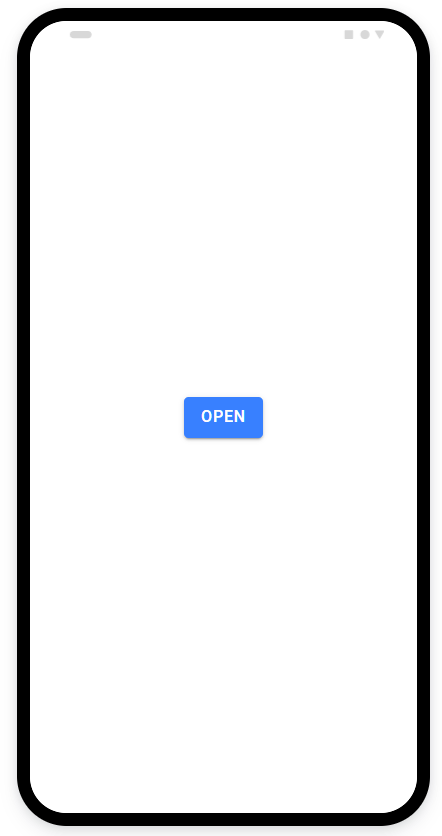
\includegraphics[scale=0.4]{Gambar/ionic-action-sheet-1.png}
        \subcaption{}
    \end{minipage}
    \begin{minipage}{0.25\linewidth}
        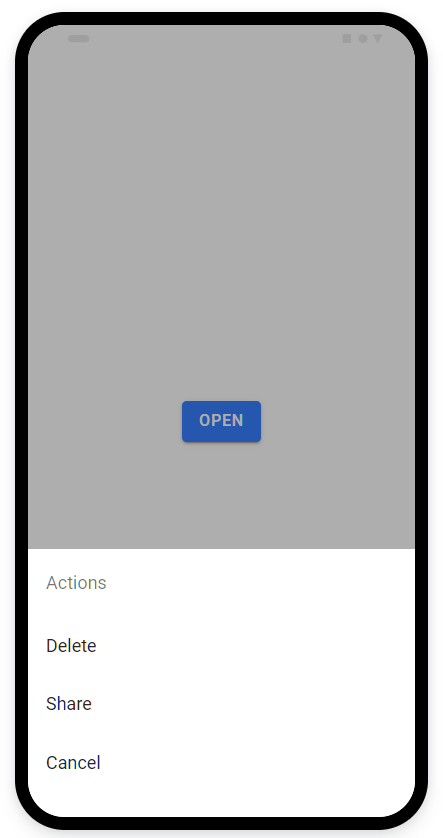
\includegraphics[scale=0.4]{Gambar/ionic-action-sheet-2.png}
        \subcaption{}
    \end{minipage}
    \caption[Gambar Hasil Action Sheet]{(a) Halaman yang hanya berisi tombol `\textit{open}', dan (b) Halaman Action Sheet ketika tombol `\textit{open}' diklik}
    \label{fig:action-sheet-example}
\end{figure}

Properti `\textit{role}' pada Action Sheet adalah sebuah properti yang diberikan untuk memberikan \textit{role} `\textit{cancel}' atau `\textit{destructive}' pada tombol yang berada di dalam Action Sheet. Nilai `\textit{cancel}' digunakan untuk tombol yang akan membatalkan aksi yang dilakukan, sedangkan nilai `\textit{destructive}' digunakan untuk tombol yang akan menghapus atau mengubah data yang ada. Selain properti role, Action Sheet memiliki properti seperti pada (Tabel \ref{tab:action-sheet-property}).

\begin{table} [H]
    \centering
    \caption{Tabel Properti dari Action Sheet}
    \begin{tabular}{|c|c|c|c|}
    \hline
       No. & Nama Properti & Deskripsi & Nilai Properti \\ \hline
        1 & animated & Memberikan animasi & `true' atau `false'\\
         &  & pada \textit{action-sheet} & \\ \hline
        2 & header & Judul untuk action-sheet & String atau undefined \\ \hline
        3 & backdrop-dissmiss & Menutup \textit{action-sheet} & `true' atau `false' \\
         &  & apabila backdrop diklik & \\ \hline
    \end{tabular}
    \label{tab:action-sheet-property}
\end{table}

\subsubsection{Button}
Button merupakan elemen interaktif yang dapat digunakan dalam berbagai aplikasi untuk menyediakan fitur tombol standar. Cara penggunaan komponen Button terdapat pada (Kode \ref{kode:ion-button}).

\begin{lstlisting}[language=HTML, caption=Contoh Potongan Kode Button, label=kode:ion-button]
<IonButton>Open</IonButton>
\end{lstlisting}

Pada komponen Button terdapat properti `\texttt{expand}' dan `\texttt{icons}'. Secara \textit{default}, komponen Button memiliki \textit{style} \texttt{display: inline-block} dan tidak memiliki ikon. Namun dengan properti \textit{expand}, \textit{style} pada komponen Button dapat diubah dengan cara memberikan properti `\texttt{expand}' pada komponen Button seperti \texttt{<IonButton expand="block">Block</IonButton>}. Properti ikon juga dapat ditambahkan pada awal, akhir, ataupun hanya terdapat ikon pada Button tersebut, seperti pada (Kode \ref{kode:ion-button-icon}). Saat menambahkan Icon, pengembang bisa mengikuti cara yang terdapat pada subbab \ref{subsubsec:icon}.

\begin{lstlisting}[language=HTML, caption=Contoh Potongan Kode Button Menggunakan Icon, label=kode:ion-button-icon]
<IonButton>
    <IonIcon slot="start" icon={star}></IonIcon>
    Left Icon
</IonButton>
\end{lstlisting}

Nilai dari `slot' dapat berupa `\texttt{start}' untuk menempatkan ikon di awal Button, `\texttt{end}' untuk menempatkan ikon di akhir button, ataupun `\texttt{icon-only}' untuk memberikan ikon saja pada button.

\subsubsection{Card}
Card merupakan komponen yang digunakan untuk menampilkan konten seperti teks, gambar, tombol, dan daftar dalam sebuah kotak. Komponen ini biasanya terdiri dari \textit{header}, judul, gambar, dan konten utama. Card dapat digunakan sebagai komponen tunggal atau digabungkan dengan komponen lain untuk membuat tampilan yang lebih kompleks. Card dapat disesuaikan dengan menggunakan properti CSS seperti `\texttt{background}' dan `\texttt{color}'. Cara menggunakan Card terdapat pada contoh (Kode \ref{kode:ion-card}).

\begin{lstlisting}[language=HTML, caption=Contoh Potongan Kode Card, label=kode:ion-card]
import React from 'react';
import { IonCard, IonCardContent, IonCardHeader, IonCardSubtitle, IonCardTitle } from '@ionic/react';

function Example() {
  return (
    <IonCard>
      <IonCardHeader>
        <IonCardTitle>Card Title</IonCardTitle>
        <IonCardSubtitle>Card Subtitle</IonCardSubtitle>
      </IonCardHeader>

      <IonCardContent>Here's a small text description for the card content. Nothing more, nothing less.</IonCardContent>
    </IonCard>
  );
}
export default Example;
\end{lstlisting}

Pengembang juga bisa menggunakan Card sebagai Media Card dengan menambahkan elemen \texttt{<img />} pada Card tersebut ataupun Button Card dengan menambahkan \texttt{<IonButton>} pada Card tersebut.

\subsubsection{Content}
Content merupakan komponen yang berguna untuk menyediakan area konten yang dapat dikontrol dan diubah menggunakan CSS. Dalam satu tampilan hanya terdapat satu konten. Konten dan komponen Ionic lainnya dapat dikostumisasi ulang dengan menggunakan CSS yang tersedia. Cara menggunakan Card terdapat pada contoh (Kode \ref{kode:ion-content}).

\begin{lstlisting}[language=HTML, caption=Contoh Potongan Kode Content, label=kode:ion-content]
import React from 'react';
import { IonContent } from '@ionic/react';

function Example() {
  return (
    <IonContent className="ion-padding">
      <h1>Heading 1</h1>

      <p>Here's a small text description for the content. Nothing more, nothing less.</p>
    </IonContent>
  );
}
export default Example;
\end{lstlisting}

Pada Content, komponen ini dapat ditambahkan header, footer. Lalu komponen content ini juga dapat berupa Fixed Content dan juga Fullscreen Content. Secara \textit{default}, Content akan memenuhi \textit{header} dan \textit{footer}.

\subsubsection{Grid}
\label{subsubsec:grid}
Komponen Grid adalah sistem \textit{layout} yang menggunakan \textit{flexbox} untuk membangun \textit{layout} yang fleksibel dan responsif. Sistem Grid ini berguna untuk mengatur ruang antara elemen pada sebuah kontainer secara dinamis berdasarkan ukuran layar dan \textit{device} yang berbeda. Pengguna dapat mengatur sendiri nilai Grid yang diinginkan. Nilai dari Grid tersebut adalah rentang angka dari 1 hingga 12. 

\subsubsection{Icon}
\label{subsubsec:icon}
Komponen Icon adalah elemen dasar yang tersedia melalui \textit{library} Ionicons. Secara \textit{default}, Icon dipersiapkan dengan semua aplikasi Ionic Framework. Komponen ini dapat digunakan untuk menampilkan ikon dari set Ionicons atau ikon yang berupa SVG. Selain itu, komponen ini juga mendukung pengaturan seperti ukuran dan warna. Cara penggunaan Icon terdapat pada (Kode \ref{kode:ion-icon}).

\begin{lstlisting}[language=HTML, caption=Contoh Kode Penggunaan Icon, label=kode:ion-icon]
import React from 'react';
import { IonIcon } from '@ionic/react';
import { logoIonic } from 'ionicons/icons';

function Example() {
  return (
    <>
      <IonIcon icon={logoIonic}></IonIcon>
      <IonIcon icon={logoIonic} size="large"></IonIcon>
      <IonIcon icon={logoIonic} color="primary"></IonIcon>
      <IonIcon icon={logoIonic} size="large" color="primary"></IonIcon>
    </>
  );
}
export default Example;
\end{lstlisting}

Untuk Icon yang diinginkan, pengembang bisa menggunakan Icon dari Ionic yang bisa didapatkan di \url{ionic.io/ionicons} ataupun bisa menambahkannya sendiri dengan cara melakukan \textit{import} pada Icon yang dimiliki.

% \subsubsection{Item}

\subsubsection{List}
List digunakan untuk menampilkan data dalam bentuk baris, seperti daftar kontak, daftar putar, atau menu. Komponen ini mendukung berbagai macam interaksi, termasuk menggeser \textit{item} untuk menampilkan opsi, menarik untuk menyusun ulang \textit{item} dalam daftar, dan menghapus \textit{item}. Komponen ini dapat ditambah berbagai elemen ke dalam daftar, seperti teks, tombol, ikon, dan gambar dengan ukuran yang kecil. Cara penggunaan List terdapat pada (Kode \ref{kode:ion-list}).

\begin{lstlisting}[language=HTML, caption=Contoh Kode Penggunaan List, label=kode:ion-list]
import React from 'react';
import { IonItem, IonLabel, IonList } from '@ionic/react';

function Example() {
  return (
    <IonList>
      <IonItem>
        <IonLabel>Pokemon Yellow</IonLabel>
      </IonItem>
      <IonItem>
        <IonLabel>Mega Man X</IonLabel>
      </IonItem>
      <IonItem>
        <IonLabel>The Legend of Zelda</IonLabel>
      </IonItem>
      <IonItem>
        <IonLabel>Pac-Man</IonLabel>
      </IonItem>
      <IonItem>
        <IonLabel>Super Mario World</IonLabel>
      </IonItem>
    </IonList>
  );
}
export default Example;
\end{lstlisting}

Komponen ini dapat ditambahkan properti `inset' untuk memberikan \textit{margin} pada tiap tepi, `lines' untuk memberikan \textit{border} bawah, dan juga `mode' untuk menentukan \textit{style} platform apa yang diinginkan. Secara \textit{default}, properti `inset' memiliki nilai `false', properti `lines' memiliki nilai `undefined', dan juga properti `mode' memiliki nilai `undefined'. Pengembang dapat mengubah nilai dari properti tersebut dengan nilai yang berada pada (Tabel \ref{tab:list-property})

\begin{table} [H]
    \centering
    \caption{Tabel Properti dari List}
    \begin{tabular}{|c|c|c|c|}
    \hline
       No. & Nama Properti & Atribut & Nilai Properti \\ \hline
        1 & inset & inset & `true' atau `false'\\ \hline
        2 & lines & lines & `full' atau `inset' atau `none'\\ \hline
        3 & mode & mode & `ios' atau `md' \\ \hline
    \end{tabular}
    \label{tab:list-property}
\end{table}

\subsubsection{Menu}
Menu merupakan \textit{navigation drawer} yang meluncur dari sisi tampilan saat dijalankan. Komponen ini adalah pola navigasi umum yang dapat secara permanen ditampilkan di layar saat diperlukan. Komponen Menu dapat digunakan untuk membuat tata letak aplikasi yang lebih terstruktur dan meningkatkan pengalaman pengguna dengan menyediakan akses mudah ke berbagai bagian dari aplikasi. Cara penggunaan Menu terdapat pada (Kode \ref{kode:ion-menu}).

\begin{lstlisting}[language=HTML, caption=Contoh Kode Penggunaan Menu, label=kode:ion-menu]
import React from 'react';
import { IonButtons, IonContent, IonHeader, IonMenu, IonMenuButton, IonPage, IonTitle, IonToolbar } from '@ionic/react';
function Example() {
  return (
    <>
      <IonMenu contentId="main-content">
        <IonHeader>
          <IonToolbar>
            <IonTitle>Menu Content</IonTitle>
          </IonToolbar>
        </IonHeader>
        <IonContent className="ion-padding">This is the menu content.</IonContent>
      </IonMenu>
      <IonPage id="main-content">
        <IonHeader>
          <IonToolbar>
            <IonButtons slot="start">
              <IonMenuButton></IonMenuButton>
            </IonButtons>
            <IonTitle>Menu</IonTitle>
          </IonToolbar>
        </IonHeader>
        <IonContent className="ion-padding">Tap the button in the toolbar to open the menu.</IonContent>
      </IonPage>
    </>
  );
}
export default Example;
\end{lstlisting}

Pada kode tersebut, halaman akan membuka \textit{side menu} ketika dipanggil. Tombol menu akan berada di kiri dikarenakan pada komponen \texttt{IonButtons}, tombol \texttt{IonMenuButtons} memiliki properti `slot' yang bernilai `start'. Secara \textit{default}, letak komponen \textit{side menu} terletak di kiri halaman. Letak dari \textit{side menu} dapat diubah dengan cara memberikan properti `side' dengan nilai `end' pada komponen \texttt{IonMenu}.

\subsubsection{Modal}
Modal dapat digunakan langsung ke dalam template. Ini mengurangi jumlah handler yang perlu dihubungkan untuk menampilkan modal.

Saat menggunakan Modal dengan Angular, React, atau Vue, komponen yang diberikan akan dihancurkan ketika modal ditutup. Fungsi ini disediakan oleh kerangka kerja JavaScript. Jika menggunakan modal tanpa kerangka kerja JavaScript, komponen yang diberikan tidak akan dihancurkan. Jika fungsi ini diperlukan, disarankan menggunakan modalController.

Contoh penggunaan Modal terdapat pada Kode \ref{kode:ion-modal}. Pada kode tersebut, Modal menggunakan properti isOpen. isOpen menggunakan binding data satu arah, yang berarti isOpen tidak akan otomatis disetel ke false saat modal ditutup. Pengembang harus mendengarkan event ionModalDidDismiss atau didDismiss dan mengatur isOpen ke false. Ini untuk mencegah bagian internal ion-modal terlalu terkait dengan status aplikasi. Dengan binding data satu arah, modal hanya perlu memperhatikan nilai boolean yang diberikan oleh variabel reaktif. Dengan binding data dua arah, modal perlu memperhatikan nilai boolean serta keberadaan variabel reaktif itu sendiri, yang dapat menyebabkan perilaku non-deterministik dan membuat aplikasi lebih sulit untuk di-debug.
\begin{lstlisting}[language=HTML, caption=Contoh Kode Penggunaan Modal, label=kode:ion-modal]
import React, { useState } from 'react';
import { IonButtons, IonButton, IonModal, IonHeader, IonContent, IonToolbar, IonTitle, IonPage } from '@ionic/react';

function Example() {
  const [isOpen, setIsOpen] = useState(false);

  return (
    <IonPage>
      <IonHeader>
        <IonToolbar>
          <IonTitle>Inline Modal</IonTitle>
        </IonToolbar>
      </IonHeader>
      <IonContent className="ion-padding">
        <IonButton expand="block" onClick={() => setIsOpen(true)}>
          Open
        </IonButton>
        <IonModal isOpen={isOpen}>
          <IonHeader>
            <IonToolbar>
              <IonTitle>Modal</IonTitle>
              <IonButtons slot="end">
                <IonButton onClick={() => setIsOpen(false)}>Close</IonButton>
              </IonButtons>
            </IonToolbar>
          </IonHeader>
          <IonContent className="ion-padding">
            <p>
              Lorem ipsum dolor sit amet consectetur adipisicing elit. Magni illum quidem recusandae ducimus quos
              reprehenderit. Veniam, molestias quos, dolorum consequuntur nisi deserunt omnis id illo sit cum qui.
              Eaque, dicta.
            </p>
          </IonContent>
        </IonModal>
      </IonContent>
    </IonPage>
  );
}

export default Example;
\end{lstlisting}

Metode yang terdapat pada Modal yaitu:
\begin{itemize}
    \item dismiss
    \begin{itemize}
        \item Deskripsi: Menutup modal setelah ditampilkan.
        \item Signature: dismiss(data?: any, role?: string) => Promise<boolean>
    \end{itemize}

    \item getCurrentBreakpoint
    \begin{itemize}
        \item Deskripsi: Mengembalikan breakpoint saat ini dari modal gaya lembar.
        \item Signature: getCurrentBreakpoint() => Promise<number | undefined>
    \end{itemize}

    \item onDidDismiss
    \begin{itemize}
        \item Deskripsi: Mengembalikan promise yang diselesaikan saat modal telah ditutup.
        \item Signature: onDidDismiss<T = any>() => Promise<OverlayEventDetail<T>>
    \end{itemize}

    \item onWillDismiss
    \begin{itemize}
        \item Deskripsi: Mengembalikan promise yang diselesaikan saat modal akan ditutup.
        \item Signature: onWillDismiss<T = any>() => Promise<OverlayEventDetail<T>>
    \end{itemize}

    \item present
    \begin{itemize}
        \item Deskripsi: Menampilkan modal setelah dibuat.
        \item Signature: present() => Promise<void>
    \end{itemize}

    \item setCurrentBreakpoint
    \begin{itemize}
        \item Deskripsi: Memindahkan modal gaya lembar ke breakpoint tertentu. Nilai breakpoint harus sesuai dengan yang didefinisikan dalam array breakpoints.
        \item Signature: setCurrentBreakpoint(breakpoint: number) => Promise<void>
    \end{itemize}
\end{itemize}

\subsubsection{Router}
\label{subbab:router}
Router digunakan untuk menangani \textit{routing} di dalam sebuah proyek JavaScript Vanilla dan Stencil. Komponen ini mengontrol semua interaksi dengan riwayat browser dan menggabungkan pembaruan melalui \texttt{ion-router-outlet}. Ion-router menggunakan sintaksis deklaratif menggunakan JSX/HTML untuk mendefinisikan pohon rute. Selain itu, \texttt{ion-router} juga memiliki lifecycle hooks dan properti untuk mengatur perilaku animasi transisi komponen. Router tidak akan pernah menyentuh DOM. Untuk menggunakan Router, pengembang dapat menggunakan \texttt{<Route>}.

\subsubsection{Toolbar}
Toolbar merupakan komponen yang digunakan untuk menampilkan judul, tombol, ikon, tombol kembali, tombol menu, kotak pencarian, segmen, dan indikator proses di aplikasi. Toolbars umumnya ditempatkan di atas atau di bawah konten dan menyediakan konten dan tindakan untuk layar saat ini. Ketika toolbar ditempatkan di \textit{header}, Toolbar akan muncul di bagian atas konten, sedangkan jika ditempatkan di \textit{footer}, Toolbar akan muncul di bagian bawah. Cara menggunakan Toolbar terdapat pada (Kode \ref{kode:ion-toolbar}).

\begin{lstlisting}[language=HTML, caption=Contoh Kode Penggunaan Toolbar, label=kode:ion-toolbar]
import React from 'react';
import { IonFooter, IonHeader, IonTitle, IonToolbar } from '@ionic/react';

function Example() {
  return (
    <>
      <IonHeader>
        <IonToolbar>
          <IonTitle>Header Toolbar</IonTitle>
        </IonToolbar>
      </IonHeader>

      <IonFooter>
        <IonToolbar>
          <IonTitle>Footer Toolbar</IonTitle>
        </IonToolbar>
      </IonFooter>
    </>
  );
}
export default Example;
\end{lstlisting}

Pada kode tersebut, Header Toolbar akan diletakan pada bagian \textit{header} dan Footer Toolbar akan diletakan pada bagian \textit{footer}. 

\subsection{Capacitor Native}
Native merupakan kemampuan untuk menambahkan fungsionalitas perangkat asli ke dalam aplikasi menggunakan \textit{plugin} API untuk Swift pada iOS, Java pada Android, dan JavaScript untuk web. Dengan menggunakan \textit{plugin} ini, pengembang dapat membuat pengalaman ``\textit{native}'' yang disesuaikan dengan mudah. Ionic menyediakan Capacitor sebagai sebuah \textit{runtime native} yang memungkinkan menambahkan fungsionalitas perangkat asli ke dalam aplikasi.

\subsubsection{Camera}
Plugin Camera pada Ionic 7 adalah sebuah plugin yang memungkinkan pengguna untuk mengambil foto dengan kamera atau memilih foto yang sudah ada dari album foto. Plugin ini dapat di-\textit{install} dengan perintah \texttt{npm install @capacitor/camera}  dan \texttt{npx cap sync}, serta menambahkan beberapa izin pada file `Info.plist' untuk iOS dan `AndroidManifest.xml' untuk Android. Selain itu, \textit{plugin} ini juga memerlukan PWA Elements agar dapat berfungsi. Cara untuk meng-\textit{install} Camera terdapat pada (Kode \ref{kode:install-camera-capacitor}), sedangkan cara untuk menggunakan Camera terdapat pada contoh (Kode \ref{kode:capacitor-cam-example}).

\begin{lstlisting}[language=HTML, caption=Kode untuk Menginstal Plugin Camera, label=kode:install-camera-capacitor]
npm install @capacitor/camera
\end{lstlisting}

\begin{lstlisting}[language=HTML, caption=Contoh Kode Capacitor Camera, label=kode:capacitor-cam-example]
import { Camera, CameraResultType } from '@capacitor/camera';

const takePicture = async () => {
  const image = await Camera.getPhoto({
    quality: 90,
    allowEditing: true,
    resultType: CameraResultType.Uri
  });

  // image.webPath will contain a path that can be set as an image src.
  // You can access the original file using image.path, which can be
  // passed to the Filesystem API to read the raw data of the image,
  // if desired (or pass resultType: CameraResultType.Base64 to getPhoto)
  var imageUrl = image.webPath;

  // Can be set to the src of an image now
  imageElement.src = imageUrl;
};
\end{lstlisting}

Pada kode tersebut, \textit{variable} `image' akan menggunakan metode \texttt{getPhoto()} di mana metode ini berfungsi untuk mengambil sebuah gambar dari album atau menangkap gambar menggunakan kamera. Properti \texttt{quality} merupakan kualitas dari gambar yang akan dikembalikan dengan nilai berikisar dari 0 hingga 100 dalam bentuk JPEG. Properti \texttt{allowEditing} berfungsi apabila pengguna ingin melakukan \textit{crop images} pada gambar. Properti \texttt{resultType} berfungsi untuk mengembalikan data dalam bentuk Base64, DataUrl, dan Uri.

\subsubsection{Filesystem}
Filesystem API menyediakan alat seperti NodeJS untuk bekerja dengan \textit{file} pada perangkat. Pengembang dapat menggunakan \textit{plugin} ini untuk melakukan operasi \textit{file} umum seperti membaca, tulis, dan mengelola isi direktori. Cara untuk meng-\textit{install} Filesystem terdapat pada (Kode \ref{kode:install-filesystem-capacitor}), sedangkan cara untuk menggunakan Filesystem terdapat pada contoh (Kode \ref{kode:example-of-filesystem-capacitor}).

\begin{lstlisting}[language=HTML, caption=Kode untuk Menginstal Plugin Filesystem, label=kode:install-filesystem-capacitor]
npm install @capacitor/action-sheet
\end{lstlisting}

\begin{lstlisting}[language=HTML, caption=Contoh Kode Penggunaan Filesystem, label=kode:example-of-filesystem-capacitor]
import { Filesystem, Directory, Encoding } from '@capacitor/filesystem';

const writeSecretFile = async () => {
  await Filesystem.writeFile({
    path: 'secrets/text.txt',
    data: 'This is a test',
    directory: Directory.Documents,
    encoding: Encoding.UTF8,
  });
};

const readSecretFile = async () => {
  const contents = await Filesystem.readFile({
    path: 'secrets/text.txt',
    directory: Directory.Documents,
    encoding: Encoding.UTF8,
  });

  console.log('secrets:', contents);
};

const deleteSecretFile = async () => {
  await Filesystem.deleteFile({
    path: 'secrets/text.txt',
    directory: Directory.Documents,
  });
};

const readFilePath = async () => {
  // Here's an example of reading a file with a full file path. Use this to
  // read binary data (base64 encoded) from plugins that return File URIs, such as
  // the Camera.
  const contents = await Filesystem.readFile({
    path: 'file:///var/mobile/Containers/Data/Application/22A433FD-D82D-4989-8BE6-9FC49DEA20BB/Documents/text.txt',
  });

  console.log('data:', contents);
};
\end{lstlisting}

\subsubsection{Preference}
Plugin Preference adalah \textit{plugin} yang berguna untuk menyimpan data sederhana dalam bentuk kunci atau nilai yang dapat diakses secara bersamaan. Preferences API menyediakan area penyimpanan data yang mendukung kunci atau nilai untuk aplikasi Ionic. Untuk menggunakan Plugin Preference dalam aplikasi Ionic, perlu meng-\textit{install plugin} Capacitor Preferences dengan cara yang terdapat pada (Kode \ref{kode:install-preference-capacitor}), sedangkan cara untuk menggunakan Capacitor terdapat pada (Kode \ref{kode:preference-capacitor-example}).

\begin{lstlisting}[language=HTML, caption=Kode untuk Menginstal Plugin Preference, label=kode:install-preference-capacitor]
npm install @capacitor/preferences
\end{lstlisting}

\begin{lstlisting}[language=HTML, caption=Contoh Kode Plugin Preference, label=kode:preference-capacitor-example]
import { Preferences } from '@capacitor/preferences';

const setName = async () => {
  await Preferences.set({
    key: 'name',
    value: 'Max',
  });
};

const checkName = async () => {
  const { value } = await Preferences.get({ key: 'name' });

  console.log(`Hello ${value}!`);
};

const removeName = async () => {
  await Preferences.remove({ key: 'name' });
};
\end{lstlisting}

% \subsection{Tabel}  
% Berikut adalah contoh pembuatan tabel. 
% Penempatan tabel dan gambar secara umum diatur secara otomatis oleh \LaTeX{}, perhatikan contoh di file bab2.tex untuk melihat bagaimana cara memaksa tabel ditempatkan sesuai keinginan kita.

% Perhatikan bawa berbeda dengan penempatan judul gambar gambar, keterangan tabel harus diletakkan di atas tabel!!
% Lihat Tabel~\ref{tab:contoh1} berikut ini:

% \begin{table}[H] %atau h saja untuk "kira kira di sini"
% 	\centering 
% 	\caption{Tabel contoh}
% 	\label{tab:contoh1}
% 	\begin{tabular}{cccc}
% 		\toprule
% 		& $v_{start}$ & $\mathcal{S}_{1}$ & $v_{end}$\\

% 		\midrule
% 		$\tau_{1}$ & 1 & 12& 20\\
% 		$\tau_{2}$ & 1 &  & 20\\
% 		$\tau_{3}$ & 1 & 9 & 20\\
% 		$\tau_{4}$ & 1 &  & 20\\

% 		\bottomrule
		
% 	\end{tabular} 
% \end{table}
% Tabel~\ref{tab:cthwarna1} dan Tabel~\ref{tab:cthwarna2} berikut ini adalah tabel dengan sel yang berwarna dan ada dua tabel yang bersebelahan. 
% \begin{table}[H]
% 	\begin{minipage}[c]{0.49\linewidth}
% 		\centering
% 		\caption{Tabel bewarna(1)}
% 		\label{tab:cthwarna1}
% 		\begin{tabular}{ccccc}
% 			\toprule
% 			 & $v_{start}$ & $\mathcal{S}_{2}$ & $\mathcal{S}_{1}$ & $v_{end}$\\
			
% 			\midrule
% 			$\tau_{1}$ & 1 & 5 \cellcolor{green}& 12& 20\\
% 			$\tau_{2}$ & 1 & 8 \cellcolor{green}& & 20\\
% 			$\tau_{3}$ & 1 & 2/8/17 \cellcolor{green}& 9 & 20\\
% 			$\tau_{4}$ & 1 & \cellcolor{red}& & 20\\
			
% 			\bottomrule

% 		\end{tabular}
% 	\end{minipage}
% 	\begin{minipage}[c]{0.49\linewidth}
		
% 		\centering 
% 		\caption{Tabel bewarna(2)}
% 		\label{tab:cthwarna2}
% 		\begin{tabular}{ccccc}
% 			\toprule
% 			 & $v_{start}$ & $\mathcal{S}_{1}$ & $\mathcal{S}_{2}$ & $v_{end}$\\
			
% 			\midrule
% 			$\tau_{1}$ & 1 & 12& 5 \cellcolor{red} &20\\
% 			$\tau_{2}$ & 1 &  &  8 \cellcolor{green} &20\\
% 			$\tau_{3}$ & 1 & 9 & 2/8/17 \cellcolor{green} &20\\
% 			$\tau_{4}$ & 1 &   & \cellcolor{red} &20\\
			
% 			\bottomrule
		
% 		\end{tabular}
% 	\end{minipage}
% \end{table}

\section{\texorpdfstring{RSS~\cite{rss-docs}}{RSS}}
RSS merupakan singkatan dari Really Simple Syndication adalah format sindikasi konten web yang merupakan dialek dari XML. Semua file RSS harus disesuaikan dengan spesifikasi XML 1.0 yang dipublikasikan oleh World Wide Web Consortium (W3C). Dokumen RSS terdiri dari elemen \texttt{<rss>} yang memiliki atribut wajib bernama version untuk menentukan versi RSS yang digunakan. Di bawah elemen \texttt{<rss>} terdapat elemen \texttt{<channel>} yang berisi informasi tentang saluran (metadata) dan isinya seperti pada (Tabel \ref{tab:elemen-rss}).
\begin{table} [H]
    \centering
    \caption{Tabel Elemen RSS}
    \begin{tabular}{|c|c|c|}
    \hline
       Element & Deskripsi & Contoh  \\ \hline
        title &  Nama dari \texttt{<channel>} & GoUpstate.com News Headlines \\ \hline
        link & URL dari web HTML yang & http://www.goupstate.com/ \\
        & berhubungan dengan \texttt{<channel>} tersebut & \\ \hline
        description & Frasa atau kalimat & The latest news from  \\ 
        & yang menjelaskan \texttt{<channel>} & GoUpstate.com, a Spartanburg \\ 
        & &  Herald-Journal Web site.\\ \hline
    \end{tabular}
    \label{tab:elemen-rss}
\end{table}

\section{\texorpdfstring{React-Axios~\cite{axios-docs}}{React-Axios}}
Package React-Axios merupakan komponen React yang menggunakan Axios untuk melakukan permintaan asinkron di dalam render. Fitur dari React-Axios yaitu:

\begin{itemize}
    \item Mewarisi semua fitur utama dari Axios.
    \item Berbasis komponen React.
    \item Menggunakan callback fungsi anak untuk menangani hasil permintaan (error, response, isLoading, makeRequest, axios).
    \item Membatalkan permintaan sebelumnya secara otomatis.
    \item Debounce untuk mencegah permintaan berulang dengan cepat.
    \item Permintaan hanya dipicu saat ada perubahan properti dan dalam keadaan siap (isReady).
    \item Mendukung callback untuk sukses (onSuccess), kesalahan (onError), dan loading (onLoading).
    \item Mendukung instance Axios kustom melalui properti atau <AxiosProvider>.
\end{itemize}

Cara untuk melakukan install package React-Axios terdapat pada Kode \ref{kode:install-react-axios}.
\begin{lstlisting}[language=Awk, caption=Kode untuk Menginstall Komponen React-Axios, label=kode:install-react-axios]
npm install react-axios
\end{lstlisting}

Komponen yang dimiliki oleh React-Axios meliputi komponen dasar dan juga komponen pembantu.

\begin{itemize}
    \item Komponen dasar: <Request> merupakan komponen dasar untuk melakukan permintaan HTTP dengan berbagai properti (instance, method, url, data, params, config, debounce, debounceImmediate, isReady, onSuccess, onLoading, onError).
    
    \item Komponen bantu: Komponen bantu yang terdapat pada React-Axios yaitu <Get>, <Delete>, <Head>, <Post>, <Put>, <Patch>. Komponen ini berfungsi untuk permintaan HTTP yang spesifik.
\end{itemize}

Contoh penggunaan React-Axios terdapat pada (Kode)

\begin{lstlisting}[language=HTML, caption=Contoh Kode dalam Melakukan GET Menggunakan React-Axios, label=kode:get-example-react-axios]
// Post a request for a user with a given ID
render() {
  return (
    <div>
      <Get url="/api/user" params={{id: "12345"}}>
        {(error, response, isLoading, makeRequest, axios) => {
          if(error) {
            return (<div>Something bad happened: {error.message} <button onClick={() => makeRequest({ params: { reload: true } })}>Retry</button></div>)
          }
          else if(isLoading) {
            return (<div>Loading...</div>)
          }
          else if(response !== null) {
            return (<div>{response.data.message} <button onClick={() => makeRequest({ params: { refresh: true } })}>Refresh</button></div>)
          }
          return (<div>Default message before request is made.</div>)
        }}
      </Get>
    </div>
  )
}
\end{lstlisting}

\section{\texorpdfstring{React Native XML to JSON Conversion~\cite{xml2js-docs}}{React Native XML to JSON Conversion}}
Package React Native XML to JSON Conversion merupakan konverter sederhana dari XML ke objek JavaScript dan mendukung konversi dua arah menggunakan sax-js dan xmlbuilder-js. Package ini diciptakan dari hasil fork pada node-xml2js yang mendukung React Native sehingga mendukung platform Android dan juga iOS. 

Cara untuk melakukan install package React-Native-XML2JS terdapat pada Kode \ref{kode:install-react-xml2js}.
\begin{lstlisting}[language=Awk, caption=Kode untuk Menginstal Komponen React-Axios, label=kode:install-react-xml2js]
npm install react-native-xml2js
\end{lstlisting}

Terdapat juga contoh penggunaan XML2JS terdapat pada Kode \ref{kode:react-xml2js-example}.
\begin{lstlisting}[language=HTML, caption=Kode Contoh Penggunaan XML2JS, label=kode:react-xml2js-example]
var parseString = require('react-native-xml2js').parseString;
var xml = "<root>Hello xml2js!</root>"
parseString(xml, function (err, result) {
    console.dir(result);
});
\end{lstlisting}

% \subsection{Kutipan}
% \label{subs:kutipan} 
% Berikut contoh kutipan dari berbagai sumber, untuk keterangan lebih lengkap, silahkan membaca file referensi.bib yang disediakan juga di template ini.
% Contoh kutipan:
% \begin{itemize}
% 	\item Buku:~\cite{berg:08:compgeom} 
% 	\item Bab dalam buku:~\cite{kreveld:04:GIS}
% 	\item Artikel dari Jurnal:~\cite{buchin:13:median}
% 	\item Artikel dari prosiding seminar/konferensi:~\cite{kreveld:11:median}
% 	\item Skripsi/Thesis/Disertasi:~\cite{lionov:02:animasi}~\cite{wiratma:10:following}~\cite{wiratma:22:later}
% 	\item Technical/Scientific Report:~\cite{kreveld:07:watertight}
% 	\item RFC (Request For Comments):~\cite{RFC1654}
% 	\item Technical Documentation/Technical Manual:~\cite{Z.500}~\cite{unicode:16:stdv9}~\cite{google:16:and7}
% 	\item Paten:~\cite{webb:12:comm}
% 	\item Tidak dipublikasikan:~\cite{wiratma:09:median}~\cite{lionov:11:cpoly}
% 	\item Laman web:~\cite{erickson:03:cgmodel}  
% 	\item Lain-lain:~\cite{agung:12:tango}
% \end{itemize}    
  
% \subsection{Gambar}

% Pada hampir semua editor, penempatan gambar di dalam dokumen \LaTeX{} tidak dapat dilakukan melalui proses {\it drag and drop}.
% Perhatikan contoh pada file bab2.tex untuk melihat bagaimana cara menempatkan gambar.
% Beberapa hal yang harus diperhatikan pada saat menempatkan gambar:
% \begin{itemize}
% 	\item Setiap gambar {\bf harus} diacu di dalam teks (gunakan {\it field} {\sc label})
% 	\item {\it Field} {\sc caption} digunakan untuk teks pengantar pada gambar. Terdapat dua bagian yaitu yang ada di antara tanda $[$ dan $]$ dan yang ada di antara tanda $\{$ dan $\}$. Yang pertama akan muncul di Daftar Gambar, sedangkan yang kedua akan muncul di teks pengantar gambar. Untuk skripsi ini, samakan isi keduanya.
% 	\item Jenis file yang dapat digunakan sebagai gambar cukup banyak, tetapi yang paling populer adalah tipe {\sc png} (lihat Gambar~\ref{fig:ularpng}), tipe {\sc jpg} (Gambar~\ref{fig:ularjpg}) dan tipe {\sc pdf} (Gambar~\ref{fig:ularpdf})
% 	\item Besarnya gambar dapat diatur dengan {\it field} {\sc scale}.
% 	\item Penempatan gambar diatur menggunakan {\it placement specifier} (di antara tanda  $[$ dan $]$ setelah deklarasi gambar.
% 	Yang umum digunakan adalah {\bf H} untuk menempatkan gambar {\bf sesuai} penempatannya di file .tex atau  {\bf h} yang berarti "kira-kira" di sini. \\
% 	Jika tidak menggunakan {\it placement specifier}, \LaTeX{} akan menempatkan gambar secara otomatis untuk menghindari bagian kosong pada dokumen anda.
% 	Walaupun cara ini sangat mudah, hindarkan terjadinya penempatan dua gambar secara berurutan. 	
% 	\begin{itemize}
% 		\item Gambar~\ref{fig:ularpng} ditempatkan di bagian atas halaman, walaupun penempatannya dilakukan setelah penulisan 3 paragraf setelah penjelasan ini.
% 		\item Gambar~\ref{fig:ularjpg} dengan skala 0.5 ditempatkan di antara dua buah paragraf. Perhatikan penulisannya di dalam file bab2.tex!
% 		\item Gambar~\ref{fig:ularpdf} ditempatkan menggunakan {\it specifier} {\bf h}.
% 	\end{itemize}
% \end{itemize}
 
% \dtext{17-18}
% \begin{figure} 
% 	\centering  
% 	\includegraphics[scale=1]{ular-png}  
% 	\caption[Gambar {\it Serpentes} dalam format png]{Gambar {\it Serpentes} dalam format png} 
% 	\label{fig:ularpng} 
% \end{figure} 

% \dtext{19-20}
% \begin{figure}[H]
% 	\centering  
% 	\includegraphics[scale=0.5]{ular-jpg}  
% 	\caption[Ular kecil]{Ular kecil} 
% 	\label{fig:ularjpg} 
% \end{figure} 
% \dtext{21-22}

% \begin{figure}[ht] 
% 	\centering  
% 	\includegraphics[scale=1]{ular-pdf}  
% 	\caption[ {\it Serpentes} betina]{ {\it Serpentes} jantan} 
% 	\label{fig:ularpdf} 
% \end{figure} 
 
% \subsection{Kode Program}

% Kode program dalam bahasa tertentu seringkali harus ditulis di dalam bab, bukan hanya dilampirkan di bagian Lampiran. 
% Kode~\ref{kode:aneh} menampilkan penggunaan karakter-karakter yang umum digunakan dalam sebuah program yang ditulis dengan bahasa C.


% \begin{lstlisting}[language=Java, caption=Kode untuk menampilkan karakter-karakter aneh, label=kode:aneh]
% // This does not make algorithmic sense, 
% // but it shows off significant programming characters.

% #include<stdio.h>

% void myFunction( int input, float* output ) {
% 	switch ( array[i] ) {
% 		case 1: // This is silly code
% 			if ( a >= 0 || b <= 3 && c != x )
% 				*output += 0.005 + 20050;
% 			char = 'g';
% 			b = 2^n + ~right_size - leftSize * MAX_SIZE;
% 			c = (--aaa + &daa) / (bbb++ - ccc % 2 );
% 			strcpy(a,"hello $@?"); 
% 	}
% 	count = ~mask | 0x00FF00AA;
% }

% // Fonts for Displaying Program Code in LATEX
% // Adrian P. Robson, nepsweb.co.uk
% // 8 October 2012
% // http://nepsweb.co.uk/docs/progfonts.pdf

% \end{lstlisting}

% \subsection{Notasi}

% Simbol-simbol (matematika) yang sering digunakan sepanjang penulisan skripsi, dapat dimasukkan ke dalam ``Daftar Notasi''. Daftar ini ada di halaman depan sebelum Bab~\ref{chap:intro}.
% Cara memasukkan sebuah simbol ke dalam Daftar Notasi adalah menggunakan perintah \verb|\nomenclature|. Contoh:
% \begin{center}
%     \verb|\nomenclature[]{$A$}{luas kandang ular}|    
% \end{center}
% \nomenclature[]{$A$}{luas kandang ular}
% \nomenclature[]{$n$}{banyaknya ular}
% \nomenclature[]{$k$}{jumlah kepala per seekor ular\nomrefpage}
% Argumen opsional digunakan untuk mengurutkan notasi. Silahkan lihat sendiri dokumentasi package \verb|nomencl|

